\documentclass{article}
\usepackage{graphicx} % Required for inserting images
\usepackage[top=0.9in, bottom=1in, left=1.5in, right=1.5in]{geometry}
\usepackage[utf8]{inputenc}
\usepackage[icelandic]{babel}
\usepackage[T1]{fontenc}
\usepackage[sc]{mathpazo}
\usepackage[parfill]{parskip}
\renewcommand{\baselinestretch}{1.2}
\usepackage{booktabs,tabularx}
\usepackage{multirow}
\usepackage{enumerate}
\usepackage{adjustbox}
\usepackage{multicol}
\usepackage{xcolor}
\usepackage{algpseudocode}
\usepackage{tikz}
\usepackage{nicefrac}
\usepackage{changepage}
\usetikzlibrary{arrows, positioning, calc, graphs}
\usepackage{amsmath, amsfonts, amssymb, amsthm}
\usepackage{graphicx}
\usepackage{tikz}
\usepackage{minted}
\usemintedstyle{manni}
\title{Forritunarmál Hópverkefni 11}
\author{Ragnar Björn Ingvarsson, rbi3}
\tikzset{->, >=stealth', shorten >=1pt, node distance=2cm,thick, main node/.style={circle,draw,minimum size=3em}}

\begin{document}
\renewcommand\thepage{}

	\maketitle

	\newpage
	\setcounter{page}{1}
	\renewcommand\thepage{\arabic{page}}

	\section{}
	\begin{minted}{haskell}
-- This loads the definition of MonadPlus:
import Control.Monad


-- Usage: let y = condMapI p f x
--        where I is one of 1,2,3,4,5,6,7,8,9,10.
-- Pre:   x is a value of type (m a) where m is
--        a monad such that (MonadPlus m) holds,
--        containing values that are valid
--        arguments for p and f. p is (a -> Bool),
--        f is (a -> b).
-- Post:  y is a value of type (m b) containing the
--        values (f z) where the z values are the
--        values in the x container such that (p z)
--        is True.

-- Only use the functions map and filter,
-- and, of course f and p. Use no other built-in
-- functions.
-- Use no list comprehension and no do-notation.
-- You should use no if-expressions.
condMap1 :: (a->Bool)->(a->b)->[a]->[b]
condMap1 p f x = map f $ filter p x

-- Use list comprehension and use no functions
-- other than f and p.
-- You should use no if-expressions.
condMap2 :: (a->Bool)->(a->b)->[a]->[b]
condMap2 p f x = [f a | a <- x, p a]

-- Use the built-in function concatMap and no other built-in
-- function. You should also use an if-expression.
condMap3 :: (a->Bool)->(a->b)->[a]->[b]
condMap3 p f x = concatMap (\x -> if p x then [f x] else []) x

-- Use do-notation and use no built-in function and
-- do not use list comprehension. You should also use
-- an if-expression.
condMap4 :: (a->Bool)->(a->b)->[a]->[b]
condMap4 p f x = do {
    let gamer []     = []
        gamer (x:xs) = if p x then (f x) : gamer xs else gamer xs
    in gamer x
}

-- Use (>>=) and return and no other built-in function.
-- You may also use the built-in special value mzero,
-- which will allow you to create a more general function
-- that works for all monads m such that (MonadPlus m)
-- holds. You should also use an if-expression.
-- The type of condMap5 may be either
--  condMap5 :: (MonadPlus m) => (a->Bool)->(a->b)->m a->m b
-- OR
condMap5 :: (a->Bool)->(a->b)->[a]->[b]
condMap5 p f x = x >>= \a -> if p a then return $ f a else mzero

-- Use (:) and no other built-in function.
-- You should not use any if-expressions.
condMap6 :: (a->Bool)->(a->b)->[a]->[b]
condMap6 _ _ [] = []
condMap6 p f (x:xs)
  | p x  = f x : condMap6 p f xs
  | True = condMap6 p f xs

-- Use head, tail and (:) and no other built-in function.
-- You should also use if-expressions.
condMap7 :: (a->Bool)->(a->b)->[a]->[b]
condMap7 p f x =
  if null x then
    []
  else
    if p $ head x then
      (f $ head x) : (condMap6 p f $ tail x)
    else
      condMap6 p f $ tail x

-- Use do-notation and use only the built-in function
-- return. Do not use any kind of list notation except [].
-- Instead of [] you may use the built-in special value
-- mzero, which will make the function more general so
-- that it works for monads m such that (MonadPlus m)
-- holds. You should also use an if-expression.
-- The type of condMap8 could be
-- condMap8 :: (a->Bool)->(a->b)->[a]->[b]
-- OR, MORE GENERAL GENERAL:
condMap8 :: MonadPlus m => (a->Bool)->(a->b)->m a->m b
condMap8 p f x = do {
    x >>= \y -> if p y then return (f y) else mzero
}

-- Use the built-in functions foldr and (:) and no
-- other built-in functions. Use no list notation
-- except []. You may use an anonymous helper function
-- and you may use if-expressions.
condMap9 :: (a->Bool)->(a->b)->[a]->[b]
condMap9 p f x = foldr (\a b -> if p a then f a:b else b) [] x

-- Use the built-in functions foldl, reverse and (:) and no
-- other built-in functions. Use no list notation
-- except []. You may use an anonymous helper function
-- and you may use if-expressions.
condMap10 :: (a->Bool)->(a->b)->[a]->[b]
condMap10 p f x = reverse (foldl (\a b -> if p b then f b:a else a) [] x)

main :: IO ()
main = do
  print (condMap1 odd (^2) [1..10])
  print (condMap2 odd (^2) [1..10])
  print (condMap3 odd (^2) [1..10])
  print (condMap4 odd (^2) [1..10])
  print (condMap5 odd (^2) [1..10])
  print (condMap6 odd (^2) [1..10])
  print (condMap7 odd (^2) [1..10])
  print (condMap8 odd (^2) [1..10])
  print (condMap9 odd (^2) [1..10])
  print (condMap10 odd (^2) [1..10])
	\end{minted}

	\begin{center}
		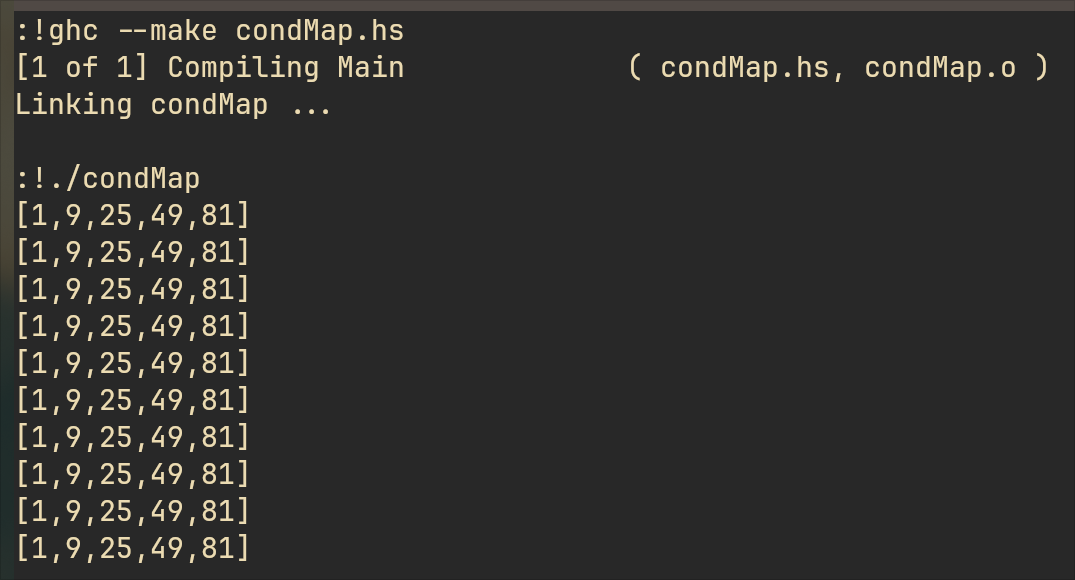
\includegraphics[scale=0.35]{hop.png}
	\end{center}
	
\end{document}
